\chapter{Partie 1 - Analyse et spécification des besoins}

\section{Objectifs de l'application, environnement, utilisateurs}

\subsection{Objectif principal}
Le principal objectif de l'application est la collecte et l'informatisation d'un maximum de données pouvant être contenues dans une facture ou un ticket de caisse.  

\subsection{Contexte}
L'application est destinée à un ou plusieurs utilisateur. Les documents à analyser peuvent être introduits sous format image (fichiers PNG, JPG, ...), PDF, ou éventuellement HTML.

\section{Contraintes de développement et performances}

\subsection{Limites en termes de terminaux et transactions simultanées}
Le nombre maximum de terminaux n’est pas pertinent dans ce projet. L’intégralité des calculs est effectuée du côté client, et la base de données est stockée localement. Si cette dernière est distante, le nombre de requêtes étant très limité, une somme importante de clients n’est pas un souci.\\

Le nombre d’accès à la base de données (partie potentiellement commune aux clients) est très réduit. De ce fait, un nombre maximum de transactions simultanées à la base de données de 1 n’est pas un problème.

\subsection{Nombre de fichiers et leurs tailles}
Pour chaque facture / ticket de caisse considéré, il y a un fichier image (jusqu’à 10 Mo), un fichier texte contenant les données récupérées (200 Ko maximum) et un autre contenant les modifications apportées par l'utilisateur (taille inférieure au premier fichier texte). Un modèle de facture / ticket de caisse doit être aussi présent pour chaque type de document ; stocké sous forme textuelle, sa taille ne dépasse pas 500 Ko.
Au total, en moyenne, pour une somme de 1000 factures, un espace de stockage de 5 Go doit être alloué.

\subsection{Temps de réponse souhaité}
Les accès à la base de données ne sont pas cruciaux en termes de durée. La lecture et l’écriture ne doivent pas être très lentes, mais un temps de réponse élevé (une seconde 
maximum) reste convenable. Cependant, la partie extraction et affichage des données ne 
doit pas être mal optimisée, car les technologies utilisées (OCR) peuvent être rapidement gourmandes en temps et capacité de calcul si elles sont poussives.

\subsection{Fiabilité et tolérance aux fautes}
La reconnaissance optique de caractères ne peut pas donner de résultats fiables pour n’importe quelle entrée. De ce fait, la partie vérification des erreurs est majoritairement réalisée par l’utilisateur, via la phase de correction et d’enregistrement dans la base de données. L’image dont les données sont extraites est aussi stockée, laissant la possibilité d’une vérification ultérieure.

Lorsqu’une urgence survient, le logiciel doit être en mesure de prévenir l’utilisateur et de ne pas transmettre de données erronées. 

\subsection{Sécurité}
Si les données présentes dans les factures sont sensibles, la mise en place de protocoles de transmission sécurisés et de chiffrage des données stockées peut être réalisée.
Certaines fonctions (notamment récupération et/ou édition d’informations présentes dans la base de données) doivent pouvoir être limitées à certains utilisateurs.\\

Comme écrit ci-dessus, certains utilisateurs peuvent n’avoir besoin que de l’affichage de certaines données. L’accès à d’autres et la modification doivent pouvoir être contrôlées, soit par des fonctions restreintes en fonction de l'utilisateur, soit par des enregistrements des activités et des vérifications de ces dernières.

Si les problèmes de sécurité discutés ci-dessus sont présents, un système de mot de passe ou de carte magnétique doit pouvoir être instauré afin de respecter les contraintes citées précédemment.

\subsection{Utilisation de standards en ce qui concerne les méthodes, outils et langages de développement.}
Le logiciel fourni doit pouvoir être portable et fonctionnel. Il doit être réutilisable et donc modulaire. Un environnement de travail à licence permissive doit être adopté, ainsi que des langages de développement libres d’utilisation.
Développé de manière portable, le logiciel devra être exécutable depuis une machine Windows ou Unix (Linux ou Mac).


\section{Analyse des besoins}
Les principales fonctions du système sont le chargement, l'extraction et la modification des données présentes dans les factures et les tickets de caisses ainsi que l'enregistrement.
\begin{figure}[h]
	\begin{center}
			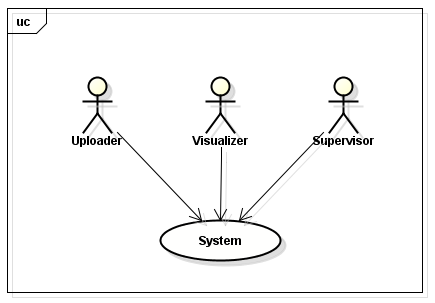
\includegraphics[scale = 0.5]{img/usecase.png}
	\end{center}
	\caption{\it Diagramme de cas d'utilisation}
	\label{usecase}

\end{figure}
\begin{enumerate}
	\item[{\bf UID :}] UC01
	\item[{\bf Name :}] Upload
	\item[{\bf Description :}]  Upload an image and apply the OCR extractor to fill the appropriate fields, modify the fields and save the file. 
	\item[{\bf Actors :}] Uploader
	\item[{\bf Initiator :}] Uploader
	\item[{\bf Pre-conditions :}]  /
	\item[{\bf Post-conditions :}]  File, extracted data and modified data saved into database. 
	\item[{\bf Flow :}]
	\begin{itemize}
		\item[{1.a.}] The uploader clicks on the button « Load Image » and choose the file.
		\item[{1.b.}] The uploader writes the path of the image
		\item[{2.}] The System tries to load the file and tests if it exists and if it is an image.
		\item[{2.a.}] [File exists and is an image]
		\begin{itemize}
			\item[{2.a.1.}] The system displays the image in the left part of the application
			\item[{2.a.2.}] The uploader selects the type of document.
			\item[{2.a.2.}] The system tries to preselect the model
			\item[{2.a.2.a}] [The model is preselected by the system]
			\begin{itemize}
				\item[{2.a.2.a.1.a.}] [The model preselected is the user choice]
			\end{itemize}
		\end{itemize}
		\item[{2.a.3.}] The uploader push the button « Extract »
		\item[{2.a.4.}] The system extracts the date from the file following the model.
		\item[{2.a.4.}] The uploader modifies the incorrect values
		\item[{2.a.4.a}] [Correct Modifications]
		\item[{2.a.5}] The uploader types a new name for the entry
		\item[{2.a.6}] The uploader saves the file
		\item[{2.a.7}] The system saves the file with the name chosen by the uploader
\smallbreak
		Alternative
		\item[{2.a.2.a.1.b.}] [The preselected model is not the user choice]
		\item[{2.a.2.a.1.b.1.}] The uploader selects another model
\smallbreak
		Alternative
		\item[{2.a.2.b}] [The Model is not preselected ]
		\begin{itemize}
			\item[{2.a.2.b.1}] The system shows the model lists
		\end{itemize}
		\item[{	2.a.2.b.2}] The uploader selects a model
\smallbreak
		Alternative
		\item[{2.b.}] [File doesn’t exist] 
		\item[{	2.b.1.}] The uploader receives an error message « The file chosen doesn’t exist».
		\begin{itemize}
			\item[{2.b.2.}] Return to 1.
		\end{itemize}
		\item[{2.c.}] [File isn’t an image] 
		\begin{itemize}
			\item[{2.b.1.}] The uploader receives an error message « The file chosen isn’t an image ».
			\item[{2.b.2.}] Return to 1. 
		\end{itemize}
\smallbreak
		Alternative
		\item[{2.a.4.b}] [Incorrect modifications]
		\begin{itemize}
			\item[{2.a.4.b.1.}] The uploader pushes the « Cancel all modifications » button 
		\end{itemize}
\smallbreak
		Exception Flow
		\item[{x.}] The uploader push the delete button
		\item[{x.1}] return to 1
	\end{itemize}
\end{enumerate}

	\newpage 
	
\begin{enumerate}	
	\item[{\bf UID :}] UC02
	\item[{\bf Name :}] Visualize
	\item[{\bf Description :}]  Visualize a file from the database
	\item[{\bf Actors :}] Visualizer
	\item[{\bf Initiator :}] Visualizer
	\item[{\bf Pre-conditions :}] / 
	\item[{\bf Post-conditions :}] /
	\item[{\bf Flow :}]
	\begin{itemize} 
		\item[{1.}]	The visualizer clicks on the « Load from database » button
		\item[{2.}]	The system shows the appropriate interface
		\item[{3.}]	The visualizer uses available filters to organize the data stored
		\item[{4.}]	The system shows the data according to the filters chosen
		\item[{5.}]	The visualizer selects the data he wants to see 
		\item[{6.}]	The system shows the data selected
		\item[{7.}]	The visualizer visualizes
		\item[{8.}]	The visualizer quits
	\end{itemize}
\end{enumerate}

\bigbreak

\begin{enumerate}
	\item[{\bf UID :}] UC03
	\item[{\bf Name :}] Supervise
	\item[{\bf Description :}]  Consult the database to obtain statistical data
	\item[{\bf Actors :}] Supervisor
	\item[{\bf Initiator :}] Supervisor
	\item[{\bf Pre-conditions :}] / 
	\item[{\bf Post-conditions :}] /
	\item[{\bf Flow :}]
	\begin{itemize} 
		\item[{1.}]	The supervisor clicks on the button « Display Statistics »
		\item[{2.}]	The system calculates and shows the current statistics
		\item[{3.}]	The supervisor visualizes
		\item[{4.}]	The supervisor quits
	\end{itemize}
\end{enumerate}

\newpage

\section{Description des scénarios}
\begin{figure}[h]
	\begin{center}
		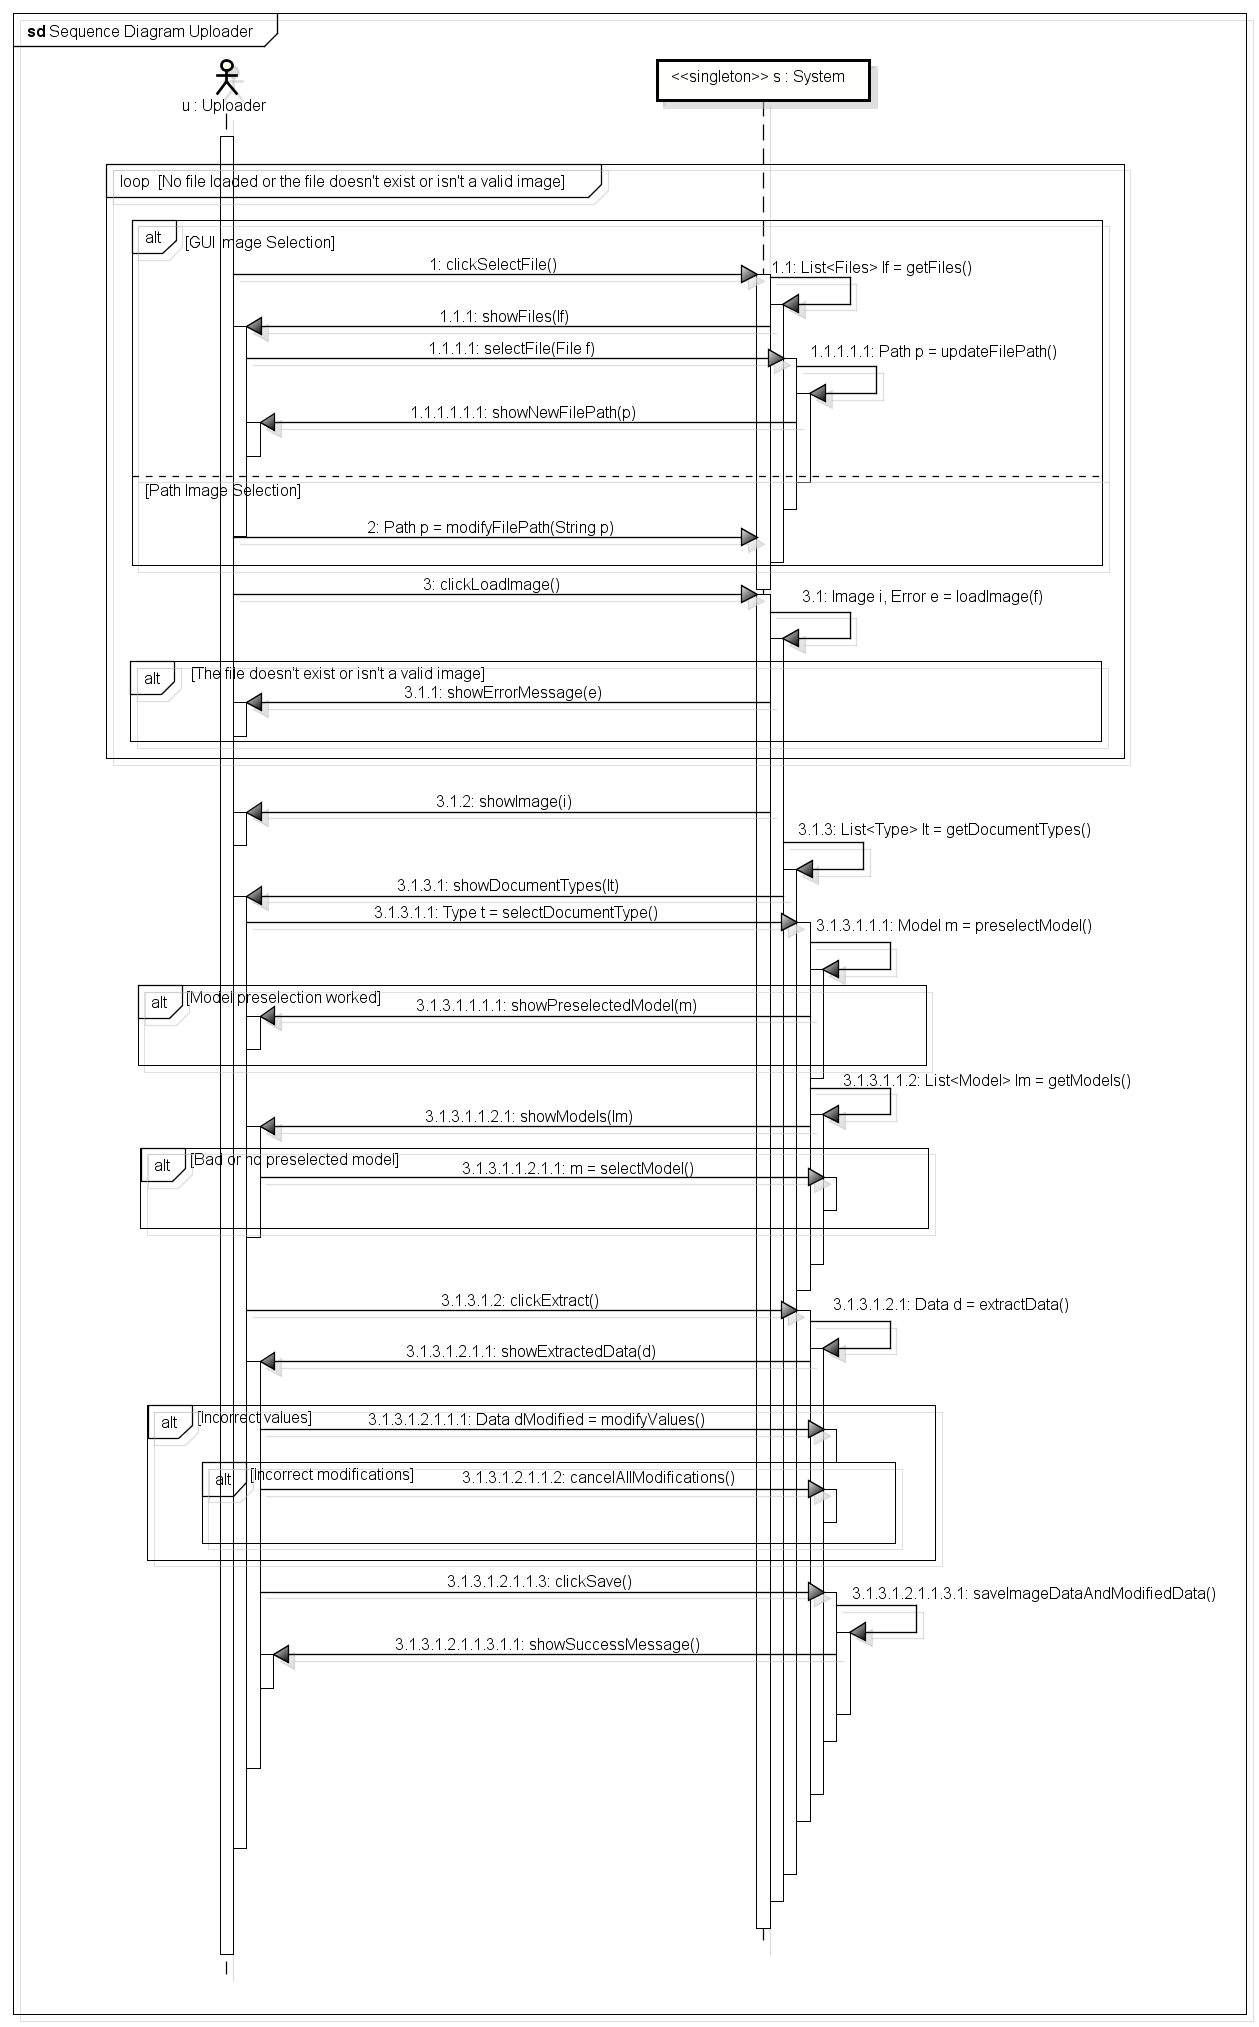
\includegraphics[scale = 0.3]{img/seqDiagUploader.png}
	\end{center}
	\caption{\it Diagramme de séquence - Chargeur}
	\label{seqDiagUploader}
\end{figure}

\begin{itemize}
	\item[{\bf UID :}] sd0
	\item[{\bf Nom :}] Diagramme de séquence Chargeur
	\item[{\bf Resumé :}]  Charge une image et procède à l'extraction des données contenues pour remplir les champs adéquats, modifie les champs erronés et enregistre le document dans la base de données (image, données extraites et données modifiées).
	\item[{\bf Acteurs :}] Chargeur
	\item[{\bf Initiateur :}] Chargeur
	\item[{\bf Pré-conditions :}]  /
	\item[{\bf Post-conditions :}]  /
\smallbreak
	\item[{\bf Description :}]
	Les fonctions propres au choix et vérifications du fichier getFiles(), showFiles() et selectFiles() sont prises en charge par l'interface elle-même. Elle est chargée d'afficher l'arborescence permettant la sélection du fichier à ouvrir. La fonction showNewFilePath() inscrit seulement le chemin du fichier sélectionné dans le champ correspondant. Le chemin peut également être entré manuellement.
	\medbreak
	Au chargement de l'image, une double vérification est effectuée : le fichier indiqué par le chemin existe-t-il , et le format de ce fichier est-il supporté par le programme. Si ces deux conditions sont vérifiées, l'image s'affiche; sinon, un message d'erreur informe l'utilisateur du problème rencontré.
	\medbreak
	S'il le peut, le système pré-sélectionne un model via showPreselectedModel().
	L'utilisateur peut choisir d'utiliser un autre modèle via selectModel(), et clique ensuite sur le bouton "Extract".
	\medbreak
	La fonction extractData() applique l'algorithme d'OCR grâce aux informations fournies par le modèle afin de remplir un maximum de champs. Les valeurs des champs sont affichées et peuvent potentiellement être modifiées par l'utilisateur.
	\medbreak
	L'utilisateur peut enregistrer les données extraites, annuler les modifications effectuées pour revenir aux données extraites brutes, ou modifié les valeurs présentent dans la base de donnée. Un message informe l'utilisateur du succès de l'opération.
\end{itemize}

 
\begin{figure}[h]
	\begin{center}
		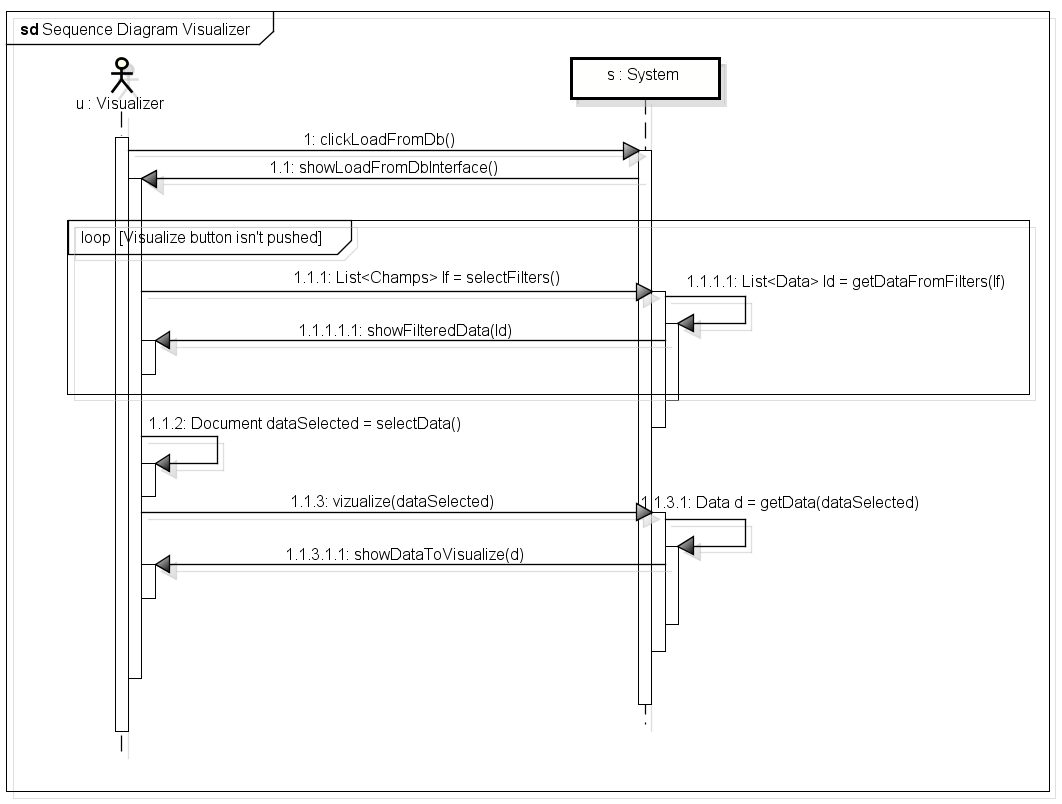
\includegraphics[scale = 0.4]{img/SeqDiagVisualizer.png}
	\end{center}
	\caption{\it Diagramme de séquence - Visualiseur}
	\label{seqDiagVisualizer}
\end{figure}

\begin{itemize}
	\item[{\bf UID :}] sd1
	\item[{\bf Nom :}] Diagramme de séquence Visualiseur
	\item[{\bf Resumé :}]  Permet de visualiser un fichier présent dans la base
	\item[{\bf Acteurs :}] Visualiseur
	\item[{\bf Initiateur :}] Visualiseur
	\item[{\bf Pré-conditions :}]  /
	\item[{\bf Post-conditions :}]  /
\smallbreak
	\item[{\bf Description :}]
	Un clic sur le bouton "LoadFromDb" appelle la fonction showLoadFormDbInterface() qui ouvre une fenêtre permettant à l'utilisateur de choisir un fichier présent dans la base de données. Un filtre permet d'affiner la recherche selon des critères particuliers appliqués aux champs.
\end{itemize}

\begin{figure}
	\begin{center}
		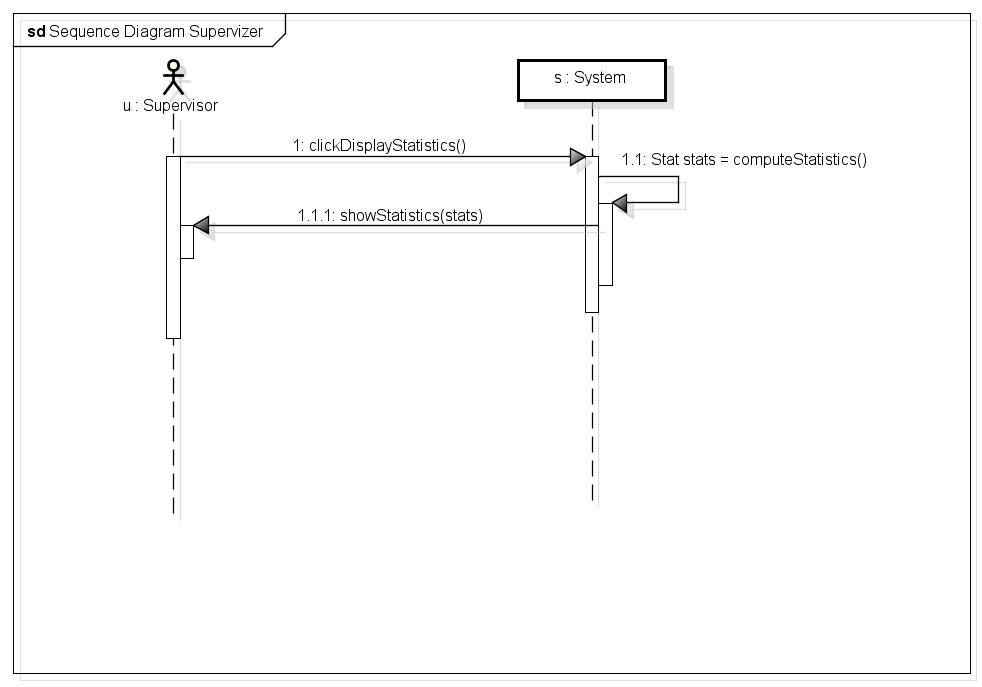
\includegraphics[scale = 0.4]{img/seqDiagSupervizer.png}
	\end{center}
	\caption{\it Diagramme de séquence - Superviseur}
	\label{seqDiagSupervizer}
\end{figure}

\begin{itemize}
	\item[{\bf UID :}] sd2
	\item[{\bf Nom :}] Diagramme de séquence Superviseur
	\item[{\bf Resumé :}]  Permet d'afficher les statistiques obtenues à partir de l'ensemble des données récoltées.
	\item[{\bf Acteurs :}] Superviseur
	\item[{\bf Initiateur :}] Superviseur
	\item[{\bf Pré-conditions :}]  /
	\item[{\bf Post-conditions :}]  /
\smallbreak
	\item[{\bf Description :}]
	Le bouton "Show Statistics" appelle la fonction clickDisplayStatistics() qui permet d'avoir des informations globales sur l'ensemble des documents analysés, voire le tracé de courbes ou de graphiques représentant l'évolution ou la répartition des données en fonction de leur type ou occurrences par exemple.
\end{itemize}

\newpage 

\section{Concepts principaux et définitions}

\begin{figure}[!h]
	\begin{center}
		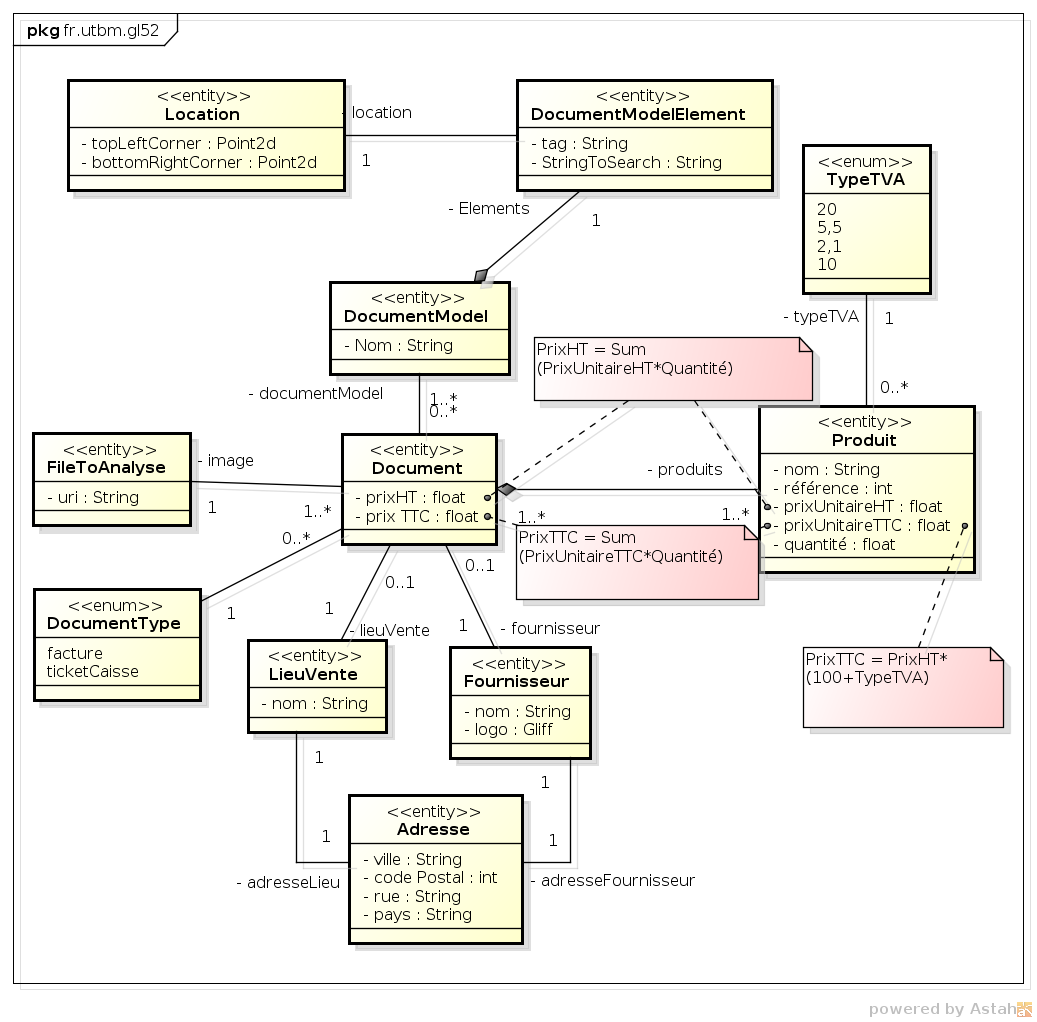
\includegraphics[scale = 0.4]{img/domainModel.png}
	\end{center}
	\caption{\it Domain Model}
	\label{domainModel}
\end{figure}

\begin{itemize}
 \item[{\bf Document :}] On appelle document l'entité enregistrée dans la base de données. Un document regroupe le fichier d'origine, l'ensemble des champs extraits par la procédure OCR, et l'ensemble des champs en tenant compte des modifications de l'utilisateur.\\
 
 \item[{\bf Modèle de facture :}] Un modèle de facture est composé de DocumentModelElement.  Dans la majorité des cas, un modèle est propre à un prestataire.\\
 
 \item[{\bf DocumentType :}] Le type de document peut être soit facture, soit ticket de caisse. Il est représenté par une enum.\\
 
 \item[{\bf DocumentModelElement :}] Chaque documentModelElement correspond à une zone d'intérêt et possède un nom qui indique le type de données contenues dans la zone, le tag. La zone elle-même est définie par un rectangle Location et/ou un mot clé StringToSearch (la donnée recherchée sera située après le mot-clé).\\
 
 \item[{\bf FileToAnalyse :}] Cette entité est un fichier physiquement présent sur le disque. Il est sélectionné par l'utilisateur et est défini par son chemin (absolu ou relatif à l'application) uri.\\
 
 \item[{\bf LieuVente :}] Un document (tel qu'une facture ou un ticket de caisse) doit comprendre plusieurs informations, telles que l'endroit où la vente a eu lieu.\\
  
 \item[{\bf Fournisseur :}] Le fournisseur est défini par son nom, prénom mais son logo peut aussi être stocké à des fins de reconnaissance automatique de modèle de document. L'émetteur de ce dernier a généralement une adresse ainsi qu'une raison sociale.\\
  
 \item[{\bf Client :}] Le client est le destinataire de la facture, défini par son nom, prénom et adresse.\\
  
 \item[{\bf Produit :}] En plus des informations uniques, un document possède obligatoirement une liste de produits achetés. Ces derniers ont chacun un nom, une référence, un prixUnitaireHT, un prixUnitaireTTC (calculé grâce au taux de TVA appliqué) ainsi qu'une quantité.\\
  
 \item[{\bf OCR :}] L'OCR, outil de reconnaissance de caractères, va permettre toute la gestion d'extraction de String à partir d'une image. Il est possible de limiter les zones de détection, et d'y associer une détection de mots clés.\\
  
 \item[{\bf Hibernate :}] Le wrapper pour Hibernate permet d'effectuer une liaison dynamique de persistance des données. Les classes dont les informations doivent être stockées dans la base de données seront converties en tables.\\
  
 \item[{\bf Controller :}] Partie du pattern Modèle Vue Contrôleur, le controller effectue la liaison entre l'interface utilisateur et les données.\\
  
 \item[{\bf GUI :}] L'interface graphique utilisateur met en place un champ d'action ergonomique, via des modules systèmes prédéfinis tels que des boutons et d'autres éléments intéractifs.
\end{itemize}


